% 2008 年福建卷文科第 22 题：椭圆 x²/a²+y²/b²=1（a>b>0），焦点 F(1,0)，过点 (2,0)。
%   AB 为垂直于 x 轴的动弦，l: x=4 与 x 轴交于 N，AF 与 BN 交于 M。
% 来源 PDF：gaokaomath-src/普通高考/2008/2008福建文.pdf
% SHA-256：185dcb32c4f56c3bc8ad4f5266794a8debebe9835bd268753a54f0b8efb6492f
% 原页：2008福建文.pdf 第 2 页（A3 三栏）第 3 栏，书页码 444。
% 重绘依据：按原页取 A 在 x≈0.7 处（B 为其关于 x 轴的对称点），F(1,0)、N(4,0)、
%   l 为 x=4 的竖直直线；AF 与 BN 的交点 M 落在 x 轴下方。
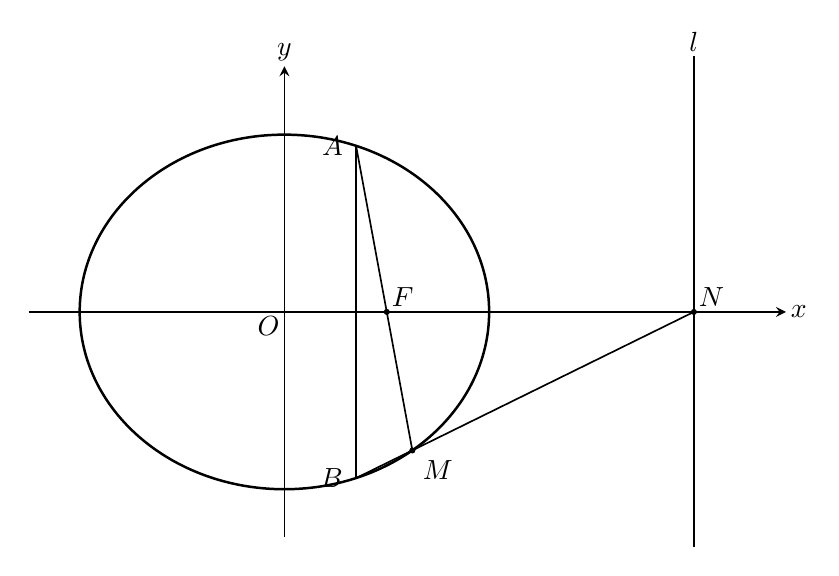
\begin{tikzpicture}[x=1.30cm, y=1.30cm, semithick, every node/.style={inner sep=1.5pt}]
  \draw[->,>=stealth] (-2.5,0) -- (4.9,0) node[right] {$x$};
  \draw[->,>=stealth] (0,-2.2) -- (0,2.4) node[above] {$y$};
  \node[below left] at (0,0) {$O$};

  \draw[line width=0.9pt] (0,0) ellipse [x radius=2, y radius=1.732];

  \coordinate (A) at (0.7,1.623);
  \coordinate (B) at (0.7,-1.623);
  \coordinate (F) at (1,0);
  \coordinate (N) at (4,0);
  \coordinate (M) at (1.25,-1.353);

  \draw (A) -- (M);
  \draw (B) -- (N);
  \draw (A) -- (B);
  \draw (4,-2.3) -- (4,2.5) node[above] {$l$};

  \fill (F) circle (1.1pt);
  \fill (M) circle (1.1pt);
  \fill (N) circle (1.1pt);

  \node[left=3pt] at (A) {$A$};
  \node[left=3pt] at (B) {$B$};
  \node[above right] at (F) {$F$};
  \node[below right=2pt] at (M) {$M$};
  \node[above right] at (N) {$N$};
\end{tikzpicture}
